\problemname{Snökaos}
Ett snöoväder har dragit in och det är kaos i trafiken.
Inte nog med det, utan vissa delar av järnvägsspåret har snöat igen vilket gjort att all tågtrafik stoppats.
Detta är naturligtvis inte så bra, eftersom mängder av resenärer nu står vid sina stationer och inte kommer någonstans.
Fredrika har därför fått i uppgift att röja bort snön mellan stationerna innan rusningstiden börjar och katastrofen är ett faktum.

Järnvägsspåret är helt utan förgreningar och har $n$ stationer, numrerade från $1$ till $n$ i den ordning de förekommer på spåret (så att station $i$ kommer precis före station $i+1$).
Det finns därmed $n - 1$ sträckor mellan stationerna.
Av dessa är $s$ täckta med snö.

Fredrika är lite orolig eftersom hon räknat ut att hon endast hinner röja bort snön från $p$ sträckor.
För att göra det bästa av situationen bestämmer sig Fredrika för att välja de sträckor som gör att så många som möjligt av de väntande resenärerna kan åka dit de vill.
Till sin hjälp har hon svaren från en enkät som hon skickat ut till alla som väntar, där de fått svara på vilka stationer de vill åka mellan.

Förutsatt att Fredrika väljer sträckorna optimalt, beräkna hur många väntande resenärer som kommer kunna åka då hon är klar.

Notera att tåg kan endast köra på snöfria sträckor. Alla stationer har tåg parkerade, så samtliga snöfria sträckor kommer att kunna trafikeras, även om stationerna inte kan nås från spårets slutstationer. Tågtrafiken är helt stoppad fram tills Fredrika är klar, så även resenärer som från början har en snöfri resväg räknas in i svaret.

\begin{figure}
	\centering
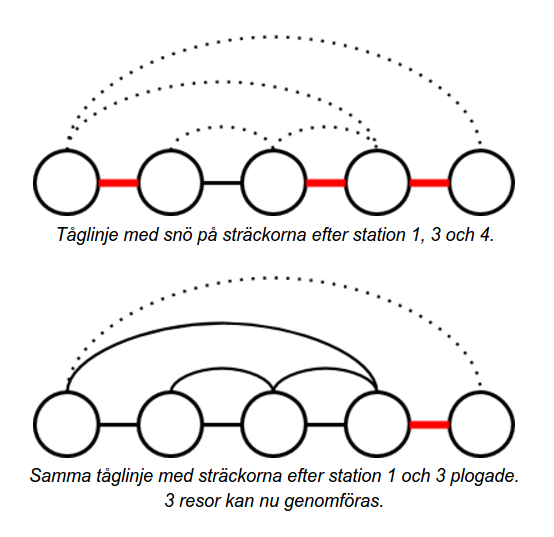
\includegraphics[width=10cm]{snokaos.png}
\caption{Sample 1}
\end{figure} 

\section*{Indata}
Första raden innehåller fyra heltal, $2 \le n \le 200$, $ 1 \le m \le 100000 $, $ 0 \le s, p \le n - 1$: antalet stationer, antalet resenärer, antalet igensnöade sträckor och antalet sträckor Fredrika hinner ploga.

Därefter följer $m$ rader där rad $i$ innehåller två heltal $1 \le a_i \not= b_i \le n$, stationerna där resenär $i$ vill starta respektive sluta.

Därefter följer $s$ rader där rad $j$ innehåller ett heltal $ 1 \le c_j \le n - 1$, stationen som ligger \emph{precis innan} den igensnöade sträckan $j$.
En sträcka förekommer högst en gång i denna lista.


\section*{Utdata}
Ditt program ska skriva ut ett enda heltal: det största antalet resenärer som kan genomföra sina resor genom att ploga högst $p$ sträckor.

\section*{Poängsättning}
Din lösning kommer att testas på en mängd testfallsgrupper. För att få poäng för en grupp så måste du klara alla testfall i gruppen.

\begin{tabular}{| l | l | l | l |}
\hline
Grupp & Poängvärde & Gränser & Övrigt \\ \hline
1     & 12         & $ n \le 200, m \le 100, p = 1$ &\\ \hline
2     & 11         & $ n \le 200, m \le 100, s \le 12 $ &\\ \hline
3     & 10          & $ n \le 200, m \le 100$ & $a_i = 1$ för alla $a_i$\\ \hline
4     & 67         & $ n \le 200$ &\\ \hline
\end{tabular}
